\begin{table}
\begin{center}
\caption{Examples of uplift events expressed and extracted from teens' microblogs.}
\begin{tabular}{l} \hline \rowcolor{gray!40}
I am really looking forward to the spring outing on Sunday now. \\ \rowcolor{gray!40}
(Doer:\emph{I}, Act:\emph{looking forward}, Object:\emph{spring outing})\\
My holiday is finally coming [smile]. \\
(Doer:\emph{My holiday}, Act:\emph{coming}, Object:\emph{[smile]})\\ \rowcolor{gray!40}%\hline
First place in my lovely math exam!!! In memory of it.\\ \rowcolor{gray!40}
Object:\emph{first place, math, exam, memory})\\ %\hline
You are always here for me like sunshine. \\
(Doer:\emph{You}, Object:\emph{sunshine})\\ \rowcolor{gray!40} %\hline
Thanks all my dear friends to take the party for me. Happiest birthday!\\ \rowcolor{gray!40}
(Doer:\emph{friends}, Act:\emph{thanks}, Object:\emph{party, birthday})\\
Be yourself. Trust yourself and follow your heart. \\
(Doer:\emph{yourself}, Act:\emph{trust}, Object:\emph{heart})\\ \rowcolor{gray!40} %\hline
Feel proud of our play in the Games. Our class is always the family!!!\\ \rowcolor{gray!40}
(Doer:\emph{Our}, Object:\emph{class, family})\\
A good film always makes bring comfort and happiness to me.\\
(Doer:\emph{me}, Act:\emph{bring}, Object:\emph{comfort, happiness})\\ \rowcolor{gray!40}%\hline
I know my mom is the one who support me forever, no matter \\ \rowcolor{gray!40}
when and where. (Doer:\emph{mom}, Act:\emph{support})\\ \hline
\end{tabular}
\label{tab:uplifts}
\end{center}
\end{table}

\begin{table}
\begin{center}
\caption{Examples of stressor events expressed and extracted from teens' microblogs.}
\begin{tabular}{l} \hline \rowcolor{gray!40}
I don't know how long can I bear the nag.\\ \rowcolor{gray!40}
(Doer:\emph{I}, Act:\emph{bear}, Object:\emph{nag})\\ %\hline
Parents like to judge everything around me with their emotion.
\\(Doer:\emph{parents}, Act:\emph{judge}, Object:\emph{everything})\\ \rowcolor{gray!40}%\hline
Hope that my uncle could revive earlier.\\ \rowcolor{gray!40}
(Doer:\emph{my uncle}, Act:\emph{revive})\\%\hline
Every one betrayed me.
\\(Doer:\emph{every one}, Act:\emph{betray}, Object:\emph{me})\\ \rowcolor{gray!40} %\hline
I'm too weak to handle such a fierce competition.\\ \rowcolor{gray!40}
(Doer:\emph{I}, Act:\emph{too weak to handle}, Object:\emph{competition})\\%\hline
I just felt hurt, depressed, self-abased and sad.
\\(Doer:\emph{I}, Act:\emph{feel hurt, depressed, self-abased and sad})\\ \rowcolor{gray!40}%\hline
My holiday is filled with all kinds of homework.\\ \rowcolor{gray!40}
(Doer:\emph{My holiday}, Act:\emph{fill with}, Object:\emph{homework})\\ %\hline
Unescapably, it's time to go back to school.
\\(Act:\emph{go back}, Object:\emph{school})\\ \rowcolor{gray!40} %\hline
When can you be aware of my heart-broken feeling again and again?\\ \rowcolor{gray!40}
(Doer:\emph{you}, Act:\emph{be aware of}, Object:\emph{heart-broken feeling})\\ \hline
\end{tabular}
\label{tab:stressors}
\end{center}
\end{table}

\begin{table}
\centering
\caption{Examples of school scheduled uplift events and stressor events.}
\label{tab:example}
\begin{tabular}{cccc}
\toprule
Type & Date	& Work Content	& Grade	\\
\midrule
\emph{stressor event} & 2014/4/16 & \emph{first day of mid-term exam} & grade1,2\\
\emph{uplift event} & 2014/11/5 & \emph{campus art festival} & grade1,2,3\\
\bottomrule
\end{tabular}
\end{table}

\begin{figure}
\centering
\caption{Examples of school related stressor events, uplift events and a student's stress fluctuation}
\includegraphics[width=\linewidth]{figs/exampleWave.eps}
\label{fig:example}
\end{figure}

\section{Data Observation}
\label{sec:obs}
We built our dataset based on two sources: 1) the microblogs of students coming from Taicang High School,
collected from January 1st, 2012 to February 1st, 2015;
and 2) list of scheduled school events, with exact start and end time.
We filtered out 124 active students according to their posting frequency from over 500 students,
and collected their microblogs throughout the whole high school career. Totally 29,232 microblogs are collected in this research,
where 236 microblogs per student on average, 1,387 microblogs maximally and 104 posts minimally.

\emph{Uplift events and stressor events}.
The list of weekly scheduled school events (from February 1st, 2012 to August 1st 2017) are collected from the school's official website
\footnote{http://stg.tcedu.com.cn/col/col82722/index.html}, with detailed event description and grade involved in the event.
There are 122 stressor events and 75 uplift events in total.
Here we give the examples of scheduled uplift and stressor events in high school life, as shown in Table~\ref{tab:example}.
There are 2-3 stressor events and 1-2 uplift event scheduled per month.


\emph{Stress detected from microblogs}.
Since our target is to observe the restoring impact of uplift events for teenagers under stress.
Based on previous research~\cite{XueUbicomp13},
we detected the stress level (ranging from 0 to 5) for each post;
and for each student, we aggregated the stress during each day by calculating the average stress of all posts.
The positive level (0-5) of each post is identified based on the frequency of positive words (see Section 5 for details).
Figure~\ref{fig:example} shows three examples of a student's stress fluctuation during three mid-term exams,
where the uplift event \emph{campus art festival} was scheduled ahead of the first exam,
the uplift event \emph{holiday} happened after the second exam,
and no scheduled uplift event was found nearby the third exam.
The current student exhibited differently in above three situations, with the stress lasting for different length and with different intensity.

To further observe the influence of uplift events for students facing stressor events,
we statistic all the stressful intervals~\cite{Li2017Analyzing} detected surround the scheduled examinations over the 124 students during their high school career.
For each student, we divide all his/her stressful intervals into two sets:
1) stressful intervals under the influence of neighbouring uplift events (e.g., \emph{Halloween activity}), and 2) independent stressful intervals.
Figure~\ref{fig:frequency} shows five measures of each student during the above two conditions:
the \emph{accumulated stress}, the \emph{average stress} (per day), the \emph{length of stressful intervals},
the \emph{frequency of academic topic words}, and the \emph{ratio of academic stress among all types of stress}.
For each measure, we calculate the average value over all eligible slides for each student.

\emph{Findings}. Comparing each measure in scheduled exam slides under the two situations: 1) existing neighbouring uplift events or 2) no neighbouring scheduled uplift events,
we find that students during exams with neighbouring uplift events exhibit less average stress intensity (both on accumulated stress and average stress),
and the length of stress slides are relatively shorter.
Further, we statistic the frequency of academic related topic words for each exam slide (as listed in Table \ref{tab:studyWords}),
and look into the ratio of academic stress among all five types of stress.
Results in Figure~\ref{fig:frequency} shows that most students talked less about the upcoming or just-finished exams when uplift events happened nearby,
with lower frequency and lower ratio.
The stress intensity and type distribution detected from each student's microblogs varies due to personal life experience, posting habits and express styles.
The statistic result shows clues about the stress-relieving ability of scheduled uplift events,
and thus helps shape our problem as how to quantify the influence of uplift events,
thus to provide further guidance for planning campus activities to help relive high school students' psychological stress effectively.

\begin{table}[h]
\centering
\caption{Examples of academic related topic words.}
\label{tab:studyWords}
\begin{tabular}{c}
\toprule
exam, fail, review, score, grade, test paper, rank, pass, math, chemistry\\
homework, recite, regress, fall behind, tension, stressed out, physics,\\
nervous, mistake, answer, question, puzzle, difficult, lesson, careless, \\
\bottomrule
\end{tabular}
\end{table}


\begin{figure}
\centering
\caption{Compare students' stress during exam intervals in two situations:
1) affected by neighboring uplift events (U-SI), 2) no uplift events occurred nearby (SI)}
\includegraphics[width=\linewidth]{figs/frequency.eps}
\label{fig:frequency}
\end{figure}

